% Created by tikzDevice version 0.10.1 on 2016-06-29 16:04:16
% !TEX encoding = UTF-8 Unicode
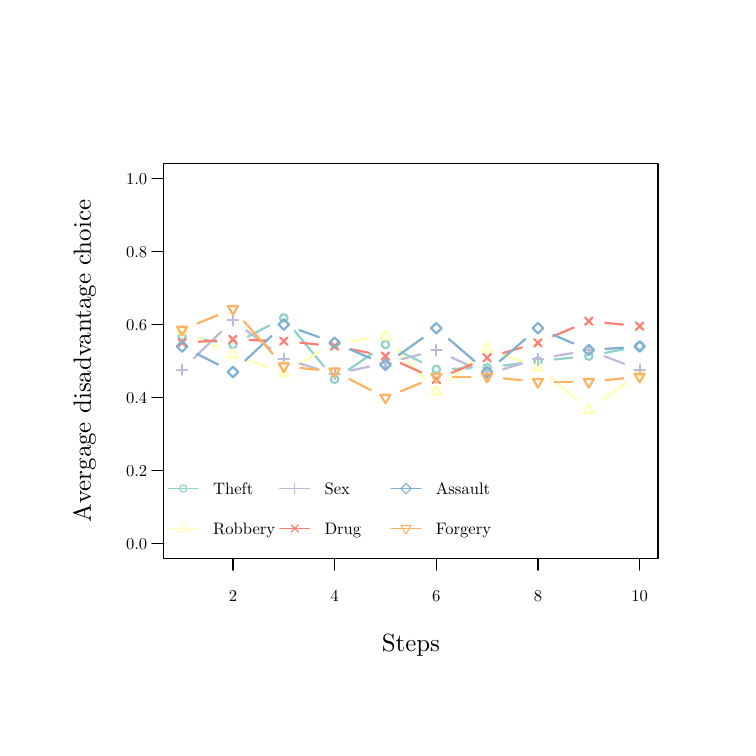
\begin{tikzpicture}[x=1pt,y=1pt]
\definecolor{fillColor}{RGB}{255,255,255}
\path[use as bounding box,fill=fillColor,fill opacity=0.00] (0,0) rectangle (252.94,252.94);
\begin{scope}
\path[clip] ( 49.20, 61.20) rectangle (227.75,203.75);
\definecolor{drawColor}{RGB}{141,211,199}

\path[draw=drawColor,line width= 0.8pt,line join=round,line cap=round] ( 61.73,140.50) -- ( 68.26,139.44);

\path[draw=drawColor,line width= 0.8pt,line join=round,line cap=round] ( 79.50,141.25) -- ( 87.23,145.29);

\path[draw=drawColor,line width= 0.8pt,line join=round,line cap=round] ( 96.38,143.45) -- (107.09,130.50);

\path[draw=drawColor,line width= 0.8pt,line join=round,line cap=round] (115.87,129.27) -- (124.34,135.08);

\path[draw=drawColor,line width= 0.8pt,line join=round,line cap=round] (134.68,135.83) -- (142.27,132.11);

\path[draw=drawColor,line width= 0.8pt,line join=round,line cap=round] (153.65,129.67) -- (160.03,129.88);

\path[draw=drawColor,line width= 0.8pt,line join=round,line cap=round] (171.98,130.85) -- (178.45,131.70);

\path[draw=drawColor,line width= 0.8pt,line join=round,line cap=round] (190.37,133.06) -- (196.79,133.69);

\path[draw=drawColor,line width= 0.8pt,line join=round,line cap=round] (208.65,135.43) -- (215.24,136.72);

\path[draw=drawColor,line width= 0.8pt,line join=round,line cap=round] ( 55.81,141.47) circle (  1.35);

\path[draw=drawColor,line width= 0.8pt,line join=round,line cap=round] ( 74.18,138.47) circle (  1.35);

\path[draw=drawColor,line width= 0.8pt,line join=round,line cap=round] ( 92.55,148.07) circle (  1.35);

\path[draw=drawColor,line width= 0.8pt,line join=round,line cap=round] (110.92,125.87) circle (  1.35);

\path[draw=drawColor,line width= 0.8pt,line join=round,line cap=round] (129.29,138.47) circle (  1.35);

\path[draw=drawColor,line width= 0.8pt,line join=round,line cap=round] (147.66,129.47) circle (  1.35);

\path[draw=drawColor,line width= 0.8pt,line join=round,line cap=round] (166.03,130.07) circle (  1.35);

\path[draw=drawColor,line width= 0.8pt,line join=round,line cap=round] (184.39,132.47) circle (  1.35);

\path[draw=drawColor,line width= 0.8pt,line join=round,line cap=round] (202.76,134.27) circle (  1.35);

\path[draw=drawColor,line width= 0.8pt,line join=round,line cap=round] (221.13,137.87) circle (  1.35);
\end{scope}
\begin{scope}
\path[clip] (  0.00,  0.00) rectangle (252.94,252.94);
\definecolor{drawColor}{RGB}{0,0,0}

\path[draw=drawColor,line width= 0.4pt,line join=round,line cap=round] ( 74.18, 61.20) -- (221.13, 61.20);

\path[draw=drawColor,line width= 0.4pt,line join=round,line cap=round] ( 74.18, 61.20) -- ( 74.18, 56.92);

\path[draw=drawColor,line width= 0.4pt,line join=round,line cap=round] (110.92, 61.20) -- (110.92, 56.92);

\path[draw=drawColor,line width= 0.4pt,line join=round,line cap=round] (147.66, 61.20) -- (147.66, 56.92);

\path[draw=drawColor,line width= 0.4pt,line join=round,line cap=round] (184.39, 61.20) -- (184.39, 56.92);

\path[draw=drawColor,line width= 0.4pt,line join=round,line cap=round] (221.13, 61.20) -- (221.13, 56.92);

\node[text=drawColor,anchor=base,inner sep=0pt, outer sep=0pt, scale=  0.60] at ( 74.18, 45.60) {2};

\node[text=drawColor,anchor=base,inner sep=0pt, outer sep=0pt, scale=  0.60] at (110.92, 45.60) {4};

\node[text=drawColor,anchor=base,inner sep=0pt, outer sep=0pt, scale=  0.60] at (147.66, 45.60) {6};

\node[text=drawColor,anchor=base,inner sep=0pt, outer sep=0pt, scale=  0.60] at (184.39, 45.60) {8};

\node[text=drawColor,anchor=base,inner sep=0pt, outer sep=0pt, scale=  0.60] at (221.13, 45.60) {10};

\path[draw=drawColor,line width= 0.4pt,line join=round,line cap=round] ( 49.20, 66.48) -- ( 49.20,198.47);

\path[draw=drawColor,line width= 0.4pt,line join=round,line cap=round] ( 49.20, 66.48) -- ( 44.92, 66.48);

\path[draw=drawColor,line width= 0.4pt,line join=round,line cap=round] ( 49.20, 92.88) -- ( 44.92, 92.88);

\path[draw=drawColor,line width= 0.4pt,line join=round,line cap=round] ( 49.20,119.27) -- ( 44.92,119.27);

\path[draw=drawColor,line width= 0.4pt,line join=round,line cap=round] ( 49.20,145.67) -- ( 44.92,145.67);

\path[draw=drawColor,line width= 0.4pt,line join=round,line cap=round] ( 49.20,172.07) -- ( 44.92,172.07);

\path[draw=drawColor,line width= 0.4pt,line join=round,line cap=round] ( 49.20,198.47) -- ( 44.92,198.47);

\node[text=drawColor,anchor=base east,inner sep=0pt, outer sep=0pt, scale=  0.60] at ( 43.20, 64.41) {0.0};

\node[text=drawColor,anchor=base east,inner sep=0pt, outer sep=0pt, scale=  0.60] at ( 43.20, 90.81) {0.2};

\node[text=drawColor,anchor=base east,inner sep=0pt, outer sep=0pt, scale=  0.60] at ( 43.20,117.21) {0.4};

\node[text=drawColor,anchor=base east,inner sep=0pt, outer sep=0pt, scale=  0.60] at ( 43.20,143.60) {0.6};

\node[text=drawColor,anchor=base east,inner sep=0pt, outer sep=0pt, scale=  0.60] at ( 43.20,170.00) {0.8};

\node[text=drawColor,anchor=base east,inner sep=0pt, outer sep=0pt, scale=  0.60] at ( 43.20,196.40) {1.0};

\path[draw=drawColor,line width= 0.4pt,line join=round,line cap=round] ( 49.20, 61.20) --
	(227.75, 61.20) --
	(227.75,203.75) --
	( 49.20,203.75) --
	( 49.20, 61.20);
\end{scope}
\begin{scope}
\path[clip] (  0.00,  0.00) rectangle (252.94,252.94);
\definecolor{drawColor}{RGB}{0,0,0}

\node[text=drawColor,anchor=base,inner sep=0pt, outer sep=0pt, scale=  0.90] at (138.47, 27.60) {Steps};

\node[text=drawColor,rotate= 90.00,anchor=base,inner sep=0pt, outer sep=0pt, scale=  0.90] at ( 22.80,132.47) {Avergage disadvantage choice};
\end{scope}
\begin{scope}
\path[clip] ( 49.20, 61.20) rectangle (227.75,203.75);
\definecolor{drawColor}{RGB}{255,255,179}

\path[draw=drawColor,line width= 0.8pt,line join=round,line cap=round] ( 61.22,140.88) -- ( 68.77,137.26);

\path[draw=drawColor,line width= 0.8pt,line join=round,line cap=round] ( 79.83,132.64) -- ( 86.90,130.10);

\path[draw=drawColor,line width= 0.8pt,line join=round,line cap=round] ( 97.70,131.16) -- (105.77,135.99);

\path[draw=drawColor,line width= 0.8pt,line join=round,line cap=round] (116.88,139.79) -- (123.33,140.56);

\path[draw=drawColor,line width= 0.8pt,line join=round,line cap=round] (133.37,136.87) -- (143.58,125.87);

\path[draw=drawColor,line width= 0.8pt,line join=round,line cap=round] (152.26,125.33) -- (161.43,133.02);

\path[draw=drawColor,line width= 0.8pt,line join=round,line cap=round] (171.67,134.84) -- (178.75,132.30);

\path[draw=drawColor,line width= 0.8pt,line join=round,line cap=round] (188.99,126.42) -- (198.17,118.73);

\path[draw=drawColor,line width= 0.8pt,line join=round,line cap=round] (207.64,118.38) -- (216.26,124.57);

\path[draw=drawColor,line width= 0.8pt,line join=round,line cap=round] ( 55.81,145.57) --
	( 57.63,142.42) --
	( 53.99,142.42) --
	( 55.81,145.57);

\path[draw=drawColor,line width= 0.8pt,line join=round,line cap=round] ( 74.18,136.77) --
	( 76.00,133.62) --
	( 72.36,133.62) --
	( 74.18,136.77);

\path[draw=drawColor,line width= 0.8pt,line join=round,line cap=round] ( 92.55,130.17) --
	( 94.37,127.02) --
	( 90.73,127.02) --
	( 92.55,130.17);

\path[draw=drawColor,line width= 0.8pt,line join=round,line cap=round] (110.92,141.17) --
	(112.74,138.02) --
	(109.10,138.02) --
	(110.92,141.17);

\path[draw=drawColor,line width= 0.8pt,line join=round,line cap=round] (129.29,143.37) --
	(131.11,140.22) --
	(127.47,140.22) --
	(129.29,143.37);

\path[draw=drawColor,line width= 0.8pt,line join=round,line cap=round] (147.66,123.57) --
	(149.48,120.42) --
	(145.84,120.42) --
	(147.66,123.57);

\path[draw=drawColor,line width= 0.8pt,line join=round,line cap=round] (166.03,138.97) --
	(167.84,135.82) --
	(164.21,135.82) --
	(166.03,138.97);

\path[draw=drawColor,line width= 0.8pt,line join=round,line cap=round] (184.39,132.37) --
	(186.21,129.22) --
	(182.58,129.22) --
	(184.39,132.37);

\path[draw=drawColor,line width= 0.8pt,line join=round,line cap=round] (202.76,116.97) --
	(204.58,113.82) --
	(200.95,113.82) --
	(202.76,116.97);

\path[draw=drawColor,line width= 0.8pt,line join=round,line cap=round] (221.13,130.17) --
	(222.95,127.02) --
	(219.31,127.02) --
	(221.13,130.17);
\definecolor{drawColor}{RGB}{190,186,218}

\path[draw=drawColor,line width= 0.8pt,line join=round,line cap=round] ( 60.11,133.55) -- ( 69.88,143.04);

\path[draw=drawColor,line width= 0.8pt,line join=round,line cap=round] ( 78.96,143.59) -- ( 87.78,136.88);

\path[draw=drawColor,line width= 0.8pt,line join=round,line cap=round] ( 98.30,131.55) -- (105.17,129.52);

\path[draw=drawColor,line width= 0.8pt,line join=round,line cap=round] (116.79,129.05) -- (123.42,130.46);

\path[draw=drawColor,line width= 0.8pt,line join=round,line cap=round] (135.10,133.17) -- (141.84,134.88);

\path[draw=drawColor,line width= 0.8pt,line join=round,line cap=round] (153.10,133.82) -- (160.59,130.34);

\path[draw=drawColor,line width= 0.8pt,line join=round,line cap=round] (171.78,129.52) -- (178.64,131.55);

\path[draw=drawColor,line width= 0.8pt,line join=round,line cap=round] (190.31,134.25) -- (196.85,135.35);

\path[draw=drawColor,line width= 0.8pt,line join=round,line cap=round] (208.37,134.22) -- (215.52,131.50);

\path[draw=drawColor,line width= 0.8pt,line join=round,line cap=round] ( 53.90,129.37) -- ( 57.72,129.37);

\path[draw=drawColor,line width= 0.8pt,line join=round,line cap=round] ( 55.81,127.46) -- ( 55.81,131.28);

\path[draw=drawColor,line width= 0.8pt,line join=round,line cap=round] ( 72.27,147.22) -- ( 76.09,147.22);

\path[draw=drawColor,line width= 0.8pt,line join=round,line cap=round] ( 74.18,145.31) -- ( 74.18,149.13);

\path[draw=drawColor,line width= 0.8pt,line join=round,line cap=round] ( 90.64,133.25) -- ( 94.46,133.25);

\path[draw=drawColor,line width= 0.8pt,line join=round,line cap=round] ( 92.55,131.34) -- ( 92.55,135.16);

\path[draw=drawColor,line width= 0.8pt,line join=round,line cap=round] (109.01,127.81) -- (112.83,127.81);

\path[draw=drawColor,line width= 0.8pt,line join=round,line cap=round] (110.92,125.90) -- (110.92,129.72);

\path[draw=drawColor,line width= 0.8pt,line join=round,line cap=round] (127.38,131.70) -- (131.20,131.70);

\path[draw=drawColor,line width= 0.8pt,line join=round,line cap=round] (129.29,129.79) -- (129.29,133.61);

\path[draw=drawColor,line width= 0.8pt,line join=round,line cap=round] (145.75,136.35) -- (149.57,136.35);

\path[draw=drawColor,line width= 0.8pt,line join=round,line cap=round] (147.66,134.45) -- (147.66,138.26);

\path[draw=drawColor,line width= 0.8pt,line join=round,line cap=round] (164.12,127.81) -- (167.93,127.81);

\path[draw=drawColor,line width= 0.8pt,line join=round,line cap=round] (166.03,125.90) -- (166.03,129.72);

\path[draw=drawColor,line width= 0.8pt,line join=round,line cap=round] (182.49,133.25) -- (186.30,133.25);

\path[draw=drawColor,line width= 0.8pt,line join=round,line cap=round] (184.39,131.34) -- (184.39,135.16);

\path[draw=drawColor,line width= 0.8pt,line join=round,line cap=round] (200.85,136.35) -- (204.67,136.35);

\path[draw=drawColor,line width= 0.8pt,line join=round,line cap=round] (202.76,134.45) -- (202.76,138.26);

\path[draw=drawColor,line width= 0.8pt,line join=round,line cap=round] (219.22,129.37) -- (223.04,129.37);

\path[draw=drawColor,line width= 0.8pt,line join=round,line cap=round] (221.13,127.46) -- (221.13,131.28);
\definecolor{drawColor}{RGB}{251,128,114}

\path[draw=drawColor,line width= 0.8pt,line join=round,line cap=round] ( 61.80,139.46) -- ( 68.19,139.88);

\path[draw=drawColor,line width= 0.8pt,line join=round,line cap=round] ( 80.18,140.08) -- ( 86.55,139.87);

\path[draw=drawColor,line width= 0.8pt,line join=round,line cap=round] ( 98.52,139.09) -- (104.95,138.46);

\path[draw=drawColor,line width= 0.8pt,line join=round,line cap=round] (116.81,136.72) -- (123.40,135.43);

\path[draw=drawColor,line width= 0.8pt,line join=round,line cap=round] (134.74,131.78) -- (142.20,128.37);

\path[draw=drawColor,line width= 0.8pt,line join=round,line cap=round] (153.18,128.22) -- (160.50,131.33);

\path[draw=drawColor,line width= 0.8pt,line join=round,line cap=round] (171.78,135.36) -- (178.64,137.38);

\path[draw=drawColor,line width= 0.8pt,line join=round,line cap=round] (189.92,141.42) -- (197.24,144.53);

\path[draw=drawColor,line width= 0.8pt,line join=round,line cap=round] (208.73,146.29) -- (215.16,145.66);

\path[draw=drawColor,line width= 0.8pt,line join=round,line cap=round] ( 54.46,137.72) -- ( 57.16,140.42);

\path[draw=drawColor,line width= 0.8pt,line join=round,line cap=round] ( 54.46,140.42) -- ( 57.16,137.72);

\path[draw=drawColor,line width= 0.8pt,line join=round,line cap=round] ( 72.83,138.92) -- ( 75.53,141.62);

\path[draw=drawColor,line width= 0.8pt,line join=round,line cap=round] ( 72.83,141.62) -- ( 75.53,138.92);

\path[draw=drawColor,line width= 0.8pt,line join=round,line cap=round] ( 91.20,138.32) -- ( 93.90,141.02);

\path[draw=drawColor,line width= 0.8pt,line join=round,line cap=round] ( 91.20,141.02) -- ( 93.90,138.32);

\path[draw=drawColor,line width= 0.8pt,line join=round,line cap=round] (109.57,136.52) -- (112.27,139.22);

\path[draw=drawColor,line width= 0.8pt,line join=round,line cap=round] (109.57,139.22) -- (112.27,136.52);

\path[draw=drawColor,line width= 0.8pt,line join=round,line cap=round] (127.94,132.92) -- (130.64,135.62);

\path[draw=drawColor,line width= 0.8pt,line join=round,line cap=round] (127.94,135.62) -- (130.64,132.92);

\path[draw=drawColor,line width= 0.8pt,line join=round,line cap=round] (146.31,124.52) -- (149.01,127.22);

\path[draw=drawColor,line width= 0.8pt,line join=round,line cap=round] (146.31,127.22) -- (149.01,124.52);

\path[draw=drawColor,line width= 0.8pt,line join=round,line cap=round] (164.68,132.32) -- (167.38,135.02);

\path[draw=drawColor,line width= 0.8pt,line join=round,line cap=round] (164.68,135.02) -- (167.38,132.32);

\path[draw=drawColor,line width= 0.8pt,line join=round,line cap=round] (183.04,137.72) -- (185.74,140.42);

\path[draw=drawColor,line width= 0.8pt,line join=round,line cap=round] (183.04,140.42) -- (185.74,137.72);

\path[draw=drawColor,line width= 0.8pt,line join=round,line cap=round] (201.41,145.52) -- (204.11,148.22);

\path[draw=drawColor,line width= 0.8pt,line join=round,line cap=round] (201.41,148.22) -- (204.11,145.52);

\path[draw=drawColor,line width= 0.8pt,line join=round,line cap=round] (219.78,143.72) -- (222.48,146.42);

\path[draw=drawColor,line width= 0.8pt,line join=round,line cap=round] (219.78,146.42) -- (222.48,143.72);
\definecolor{drawColor}{RGB}{128,177,211}

\path[draw=drawColor,line width= 0.8pt,line join=round,line cap=round] ( 61.17,135.06) -- ( 68.82,131.21);

\path[draw=drawColor,line width= 0.8pt,line join=round,line cap=round] ( 78.57,132.61) -- ( 88.17,141.58);

\path[draw=drawColor,line width= 0.8pt,line join=round,line cap=round] ( 98.20,143.64) -- (105.27,141.10);

\path[draw=drawColor,line width= 0.8pt,line join=round,line cap=round] (116.43,136.70) -- (123.78,133.53);

\path[draw=drawColor,line width= 0.8pt,line join=round,line cap=round] (134.16,134.65) -- (142.78,140.85);

\path[draw=drawColor,line width= 0.8pt,line join=round,line cap=round] (152.20,140.43) -- (161.48,132.43);

\path[draw=drawColor,line width= 0.8pt,line join=round,line cap=round] (170.57,132.43) -- (179.85,140.43);

\path[draw=drawColor,line width= 0.8pt,line join=round,line cap=round] (189.90,141.98) -- (197.25,138.81);

\path[draw=drawColor,line width= 0.8pt,line join=round,line cap=round] (208.75,136.86) -- (215.15,137.32);

\path[draw=drawColor,line width= 0.8pt,line join=round,line cap=round] ( 53.90,137.75) --
	( 55.81,139.66) --
	( 57.72,137.75) --
	( 55.81,135.84) --
	( 53.90,137.75);

\path[draw=drawColor,line width= 0.8pt,line join=round,line cap=round] ( 72.27,128.51) --
	( 74.18,130.42) --
	( 76.09,128.51) --
	( 74.18,126.60) --
	( 72.27,128.51);

\path[draw=drawColor,line width= 0.8pt,line join=round,line cap=round] ( 90.64,145.67) --
	( 92.55,147.58) --
	( 94.46,145.67) --
	( 92.55,143.76) --
	( 90.64,145.67);

\path[draw=drawColor,line width= 0.8pt,line join=round,line cap=round] (109.01,139.07) --
	(110.92,140.98) --
	(112.83,139.07) --
	(110.92,137.16) --
	(109.01,139.07);

\path[draw=drawColor,line width= 0.8pt,line join=round,line cap=round] (127.38,131.15) --
	(129.29,133.06) --
	(131.20,131.15) --
	(129.29,129.24) --
	(127.38,131.15);

\path[draw=drawColor,line width= 0.8pt,line join=round,line cap=round] (145.75,144.35) --
	(147.66,146.26) --
	(149.57,144.35) --
	(147.66,142.44) --
	(145.75,144.35);

\path[draw=drawColor,line width= 0.8pt,line join=round,line cap=round] (164.12,128.51) --
	(166.03,130.42) --
	(167.93,128.51) --
	(166.03,126.60) --
	(164.12,128.51);

\path[draw=drawColor,line width= 0.8pt,line join=round,line cap=round] (182.49,144.35) --
	(184.39,146.26) --
	(186.30,144.35) --
	(184.39,142.44) --
	(182.49,144.35);

\path[draw=drawColor,line width= 0.8pt,line join=round,line cap=round] (200.85,136.43) --
	(202.76,138.34) --
	(204.67,136.43) --
	(202.76,134.52) --
	(200.85,136.43);

\path[draw=drawColor,line width= 0.8pt,line join=round,line cap=round] (219.22,137.75) --
	(221.13,139.66) --
	(223.04,137.75) --
	(221.13,135.84) --
	(219.22,137.75);
\definecolor{drawColor}{RGB}{253,180,98}

\path[draw=drawColor,line width= 0.8pt,line join=round,line cap=round] ( 61.36,146.06) -- ( 68.63,149.05);

\path[draw=drawColor,line width= 0.8pt,line join=round,line cap=round] ( 78.16,146.84) -- ( 88.57,135.08);

\path[draw=drawColor,line width= 0.8pt,line join=round,line cap=round] ( 98.52,129.97) -- (104.95,129.31);

\path[draw=drawColor,line width= 0.8pt,line join=round,line cap=round] (116.26,125.96) -- (123.95,122.01);

\path[draw=drawColor,line width= 0.8pt,line join=round,line cap=round] (134.84,121.55) -- (142.11,124.54);

\path[draw=drawColor,line width= 0.8pt,line join=round,line cap=round] (153.66,126.82) -- (160.03,126.82);

\path[draw=drawColor,line width= 0.8pt,line join=round,line cap=round] (171.99,126.20) -- (178.43,125.54);

\path[draw=drawColor,line width= 0.8pt,line join=round,line cap=round] (190.39,124.93) -- (196.76,124.93);

\path[draw=drawColor,line width= 0.8pt,line join=round,line cap=round] (208.73,125.54) -- (215.16,126.20);

\path[draw=drawColor,line width= 0.8pt,line join=round,line cap=round] ( 55.81,141.69) --
	( 57.63,144.84) --
	( 53.99,144.84) --
	( 55.81,141.69);

\path[draw=drawColor,line width= 0.8pt,line join=round,line cap=round] ( 74.18,149.23) --
	( 76.00,152.38) --
	( 72.36,152.38) --
	( 74.18,149.23);

\path[draw=drawColor,line width= 0.8pt,line join=round,line cap=round] ( 92.55,128.49) --
	( 94.37,131.64) --
	( 90.73,131.64) --
	( 92.55,128.49);

\path[draw=drawColor,line width= 0.8pt,line join=round,line cap=round] (110.92,126.60) --
	(112.74,129.75) --
	(109.10,129.75) --
	(110.92,126.60);

\path[draw=drawColor,line width= 0.8pt,line join=round,line cap=round] (129.29,117.17) --
	(131.11,120.32) --
	(127.47,120.32) --
	(129.29,117.17);

\path[draw=drawColor,line width= 0.8pt,line join=round,line cap=round] (147.66,124.72) --
	(149.48,127.87) --
	(145.84,127.87) --
	(147.66,124.72);

\path[draw=drawColor,line width= 0.8pt,line join=round,line cap=round] (166.03,124.72) --
	(167.84,127.87) --
	(164.21,127.87) --
	(166.03,124.72);

\path[draw=drawColor,line width= 0.8pt,line join=round,line cap=round] (184.39,122.83) --
	(186.21,125.98) --
	(182.58,125.98) --
	(184.39,122.83);

\path[draw=drawColor,line width= 0.8pt,line join=round,line cap=round] (202.76,122.83) --
	(204.58,125.98) --
	(200.95,125.98) --
	(202.76,122.83);

\path[draw=drawColor,line width= 0.8pt,line join=round,line cap=round] (221.13,124.72) --
	(222.95,127.87) --
	(219.31,127.87) --
	(221.13,124.72);
\definecolor{drawColor}{RGB}{141,211,199}

\path[draw=drawColor,line width= 0.4pt,line join=round,line cap=round] ( 50.82, 86.40) -- ( 61.62, 86.40);
\definecolor{drawColor}{RGB}{255,255,179}

\path[draw=drawColor,line width= 0.4pt,line join=round,line cap=round] ( 50.82, 72.00) -- ( 61.62, 72.00);
\definecolor{drawColor}{RGB}{190,186,218}

\path[draw=drawColor,line width= 0.4pt,line join=round,line cap=round] ( 91.07, 86.40) -- (101.87, 86.40);
\definecolor{drawColor}{RGB}{251,128,114}

\path[draw=drawColor,line width= 0.4pt,line join=round,line cap=round] ( 91.07, 72.00) -- (101.87, 72.00);
\definecolor{drawColor}{RGB}{128,177,211}

\path[draw=drawColor,line width= 0.4pt,line join=round,line cap=round] (131.32, 86.40) -- (142.12, 86.40);
\definecolor{drawColor}{RGB}{253,180,98}

\path[draw=drawColor,line width= 0.4pt,line join=round,line cap=round] (131.32, 72.00) -- (142.12, 72.00);
\definecolor{drawColor}{RGB}{141,211,199}

\path[draw=drawColor,line width= 0.4pt,line join=round,line cap=round] ( 56.22, 86.40) circle (  1.35);
\definecolor{drawColor}{RGB}{255,255,179}

\path[draw=drawColor,line width= 0.4pt,line join=round,line cap=round] ( 56.22, 74.10) --
	( 58.04, 70.95) --
	( 54.40, 70.95) --
	( 56.22, 74.10);
\definecolor{drawColor}{RGB}{190,186,218}

\path[draw=drawColor,line width= 0.4pt,line join=round,line cap=round] ( 94.56, 86.40) -- ( 98.38, 86.40);

\path[draw=drawColor,line width= 0.4pt,line join=round,line cap=round] ( 96.47, 84.49) -- ( 96.47, 88.31);
\definecolor{drawColor}{RGB}{251,128,114}

\path[draw=drawColor,line width= 0.4pt,line join=round,line cap=round] ( 95.12, 70.65) -- ( 97.82, 73.35);

\path[draw=drawColor,line width= 0.4pt,line join=round,line cap=round] ( 95.12, 73.35) -- ( 97.82, 70.65);
\definecolor{drawColor}{RGB}{128,177,211}

\path[draw=drawColor,line width= 0.4pt,line join=round,line cap=round] (134.81, 86.40) --
	(136.72, 88.31) --
	(138.63, 86.40) --
	(136.72, 84.49) --
	(134.81, 86.40);
\definecolor{drawColor}{RGB}{253,180,98}

\path[draw=drawColor,line width= 0.4pt,line join=round,line cap=round] (136.72, 69.90) --
	(138.53, 73.05) --
	(134.90, 73.05) --
	(136.72, 69.90);
\definecolor{drawColor}{RGB}{0,0,0}

\node[text=drawColor,anchor=base west,inner sep=0pt, outer sep=0pt, scale=  0.60] at ( 67.02, 84.33) {Theft};

\node[text=drawColor,anchor=base west,inner sep=0pt, outer sep=0pt, scale=  0.60] at ( 67.02, 69.93) {Robbery};

\node[text=drawColor,anchor=base west,inner sep=0pt, outer sep=0pt, scale=  0.60] at (107.27, 84.33) {Sex};

\node[text=drawColor,anchor=base west,inner sep=0pt, outer sep=0pt, scale=  0.60] at (107.27, 69.93) {Drug};

\node[text=drawColor,anchor=base west,inner sep=0pt, outer sep=0pt, scale=  0.60] at (147.52, 84.33) {Assault};

\node[text=drawColor,anchor=base west,inner sep=0pt, outer sep=0pt, scale=  0.60] at (147.52, 69.93) {Forgery};
\end{scope}
\end{tikzpicture}
